\section{Komunikační řetězec, vrstvový model datového přenosu, základní operace při zpracování signálu u digitálního komunikačního systému. Úrovně signálu a vztažné hodnoty, absolutní a relativní úroveň, útlum, zisk, odstup signálu od šumu, výkonová spektrální hustota, přenosová kapacita kanálu.
}

\subsection{Komunikační řetězec}

\begin{figure}[h]
    \centering
	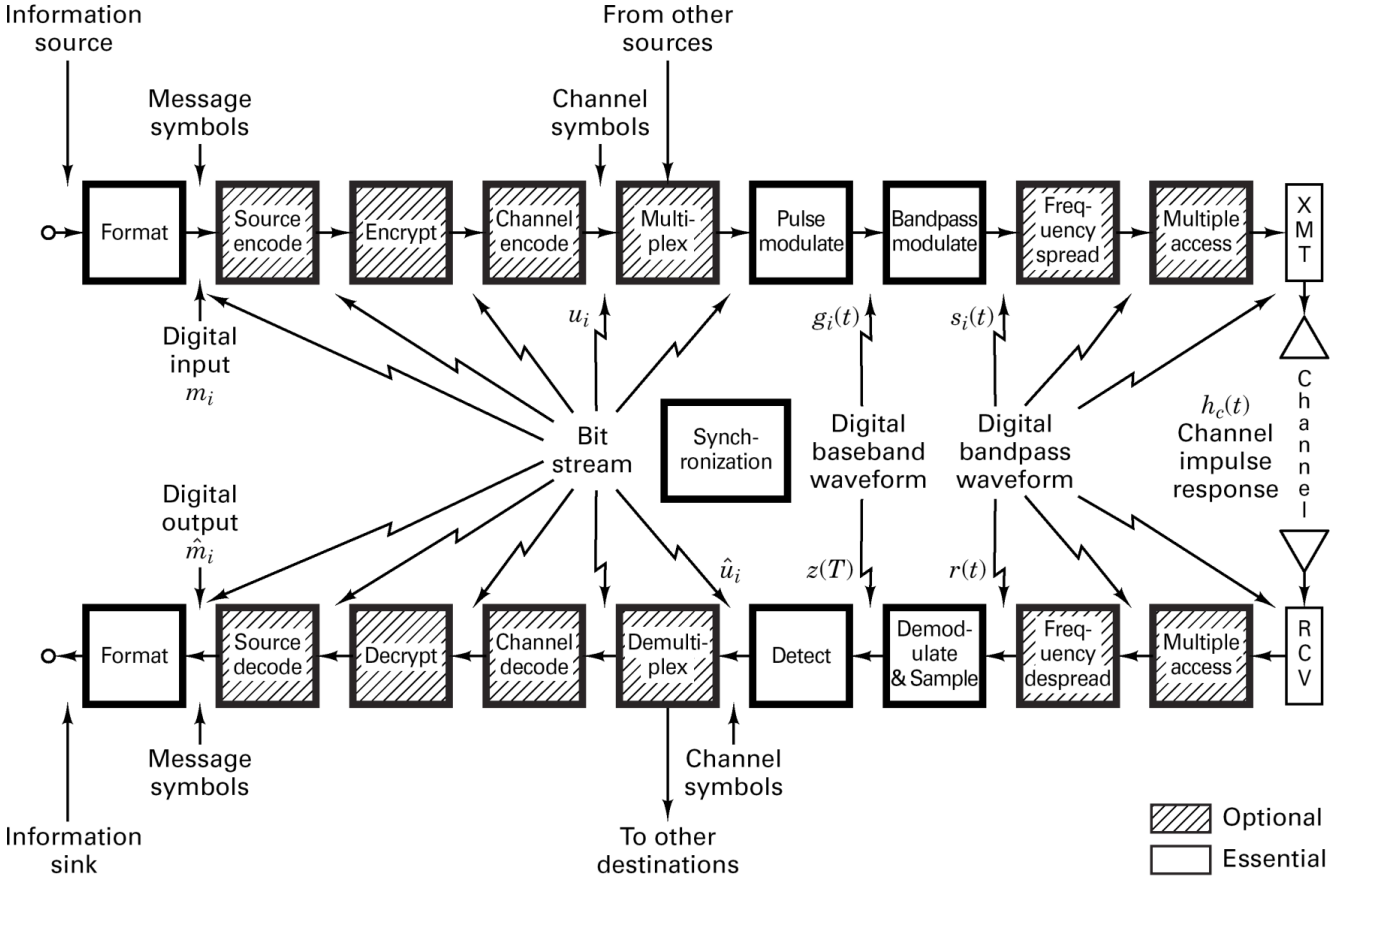
\includegraphics[width=0.9\textwidth]{images/010.png}
    \caption{Komunikační řetězec}
    \label{komStr}
\end{figure}

\subsection{Základní operace}

\textbf{Format -- digitalizace signálu}: vzorkování, lineární a nelineární kvantování, pulzně kódová modulace.
\newline\textbf{Source encode -- zdrojové kódování}: kódování řeči, hudby a obrazu pro odstranění redundance, ztrátové (JPEG, MPEG) a bezeztrátové (Huffman) kódování.
\newline\textbf{Encrypt -- šifrování}: zabezpečení dat proti zneužití, symetrické a asymetrické systémy.
\newline\textbf{Channel encode -- kanálové kódování}: zabezpečení dat proti chybám (detekční nebo opravné kódy).
\newline\textbf{Multiplex}: sloučení více datových toků od více uživatelů do jednoho.
\newline\textbf{Pulse modulate -- tvarování pulzů}: tvarování pulsů za účelem snížení šířky pásma a potlačení mezisymbolových interferencí
\newline\textbf{Bandpass modulate -- modulace}: převod signálu ze základního pásma do přenosového. Různé modulace (MQAM, MPSK, MFSK, GMSK, ...).
\newline\textbf{Frequency spread -- kmitočtové rozprostření}: rozšíření kmitočtového spektra pro širokopásmové přenosy (eliminace úniků).
\newline\textbf{Multiple access -- mnohonásobný přístup}: metody přístupu -- časové (TDMA), kmitočtové (FDMA), kódové (CDMA), prostorové (SDMA), polarizační (PDMA).
\newline\textbf{XMT -- vysílač}
\newline\textbf{Synchronization -- synchronizace}: slouží pro zajištění přenosu, získání informace o časování symbolů, kmitočtu a fázi nosné vlny, časování rámců a další.
\newline\textbf{Channel -- přenosový kanál}: rušivé vlivy -- zpoždění rušení a další.
\newline\textbf{RCV -- přijímač}
\newline\textbf{Demodulate \& Sample -- demudulace a vzorkování}: převod signálu demodulátorem do základního pásma, ekvalizace a vzorkování ve vhodných okamžicích daných synchronizací.
\newline\textbf{Detect -- vyhodnocení symbolů}: detekce symbolů v závislosti na typu modulace.

\subsection{Úroveň signálu a vztažné hodnoty}
\textbf{Relativní úrovně} -- vztažné k úrovni ve vztažném místě 0. $P_0$ a $U_0$ je vztažný výkon respektive vztažné napětí ve vztažném bodě 0.
\[L_r=10*\log\frac{P_x}{P_0} \quad [dBr; W, W]\]
\[L_{ru}=20*\log\frac{U_x}{U_0} \quad [dBru; V, V]\]

\textbf{Absolutní úrovně} jsou vztažné k referenční hodnotě, tj. že za vztažné hodnoty se dosazuje referenční hodnota (např. $P_0 = 0,001$ Mw). Z je označení impedance.
\[L_m = 10*\log\frac{P}{P_0} = 10*\log\frac{\frac{U^2}{Z}}{\frac{P^2_0}{Z_0}} = 20*\log\frac{U}{U_0} + 10*\log\frac{Z}{Z_0} = L_u + \Delta Z\]

\textbf{Útlum (A)} se vypočítá jako $A = L_{m1} - L_{m2}$.
\newline\textbf{Zisk (G)} také označován jako \textbf{S} je opakem útlumu.
\newline\textbf{SNR -- odstup signál šum} -- je podíl výkonu signálu (S) k výkonu šumu (N)\[SNR = \frac{S}{N}\] nebo \[SNR = 10*\log_{10}\frac{S}{N} = 20*\log_{10}\frac{U_s}{U_n} \quad [dB, W, W, V, V]\]

\textbf{PSD -- výkonová spektrální hustota} udává rozložení výkonu při přenosu signálů s náhodným charakterem -- spojité kmitočtové spektrum. \[PSD = \frac{P}{B} \quad [W/Hz, W, Hz]\] kde B je šířka pásma.

\textbf{Přenosová kapacita kanálu} -- Maximální rychlost přenosu se nazývá kapacita kanálu (C). To je množství informace které lze přenést za jednotku času. Shannon-Hartley teorém
\[C = B*\log_2(1 + \frac{S}{N}) \quad [b/s, Hz, W, W]\]
\[C = 3,32B*\log_10(1 + \frac{S}{N})\]
\[C = \int\limits_B{\log_2\left[1 + \frac{S(f)}{N(f)}\right]df}\]


\clearpage
\section{Princip zvyšování odolnosti přenášené zprávy proti chybám, informační poměr kódu, Hammingova vzdálenost, podmínky možnosti detekce a korekce chyb.}

\subsection{Princip}

Pro protichybové zabezpečení spočívá ve zvětšení bitové nadbytečnosti například pomocí zabezpečovacích kódů. Data se rozdělí na bloky a ke každému bloku jsou doplněny kontrolní bity.

Existují:
\begin{itemize}
    \item Detekční kódy - detekují chybu (využití ARQ)
    \item Korelační kódy - detekují a opravují chybu (využití FEC)
\end{itemize}

Chyby lze dělit na:
\begin{itemize}
    \item Nezávislé chyby
    \item Shluky chyb
\end{itemize}

Zpráva je zabezpečována po úsecích délky \textit{k}, kde k je délka informačního slova.
Přidané zabezpečovací bity se označují jako \textit{r} a jsou odvozeny z informačního slova.
Součtem \textit{k} a \textit{r} vznikne kódové slovo \textit{n}.

Jestliže je zabezpečovací část připojena hned za informační část kód je systematický.
V případě že informační a zabezpečující bity jsou promíchány tak je kód nesystematický.

\subsection{Informační poměr kódu}

Informační poměr kódu se vypočte jako $R=\frac{n-r}{n}$.
Informační poměr kódu se označuje jako kód \textit{(n, k)}, kdy to zároveň určuje jeho parametry.


Na ukázce je tabulka pro informační poměl kódu (4, 2). Výsledný informační poměr po dosazení $R = 0,5$.

\begin{table}[ht]
    \centering
    \begin{tabular}{|c|c|}
        \hline
        Informační slovo & Kódové slovo \\\hline
        00 & 0000 \\\hline
        01 & 0110 \\\hline
        10 & 1001 \\\hline
        11 & 1111 \\\hline
    \end{tabular}
\end{table}

Výsledkem jsou 4 kódová slova i když existuje celkem 16 možných variant.
Výběr těchto slov je volen aby bylo možné detekovat a opravovat chyby podle určitého kritéria.

Parametry:
\begin{itemize}
    \item Délka kódu L -- počet všech různých kódových slov
    \item Hammingova váha $w(v)$ -- počet jedniček v kódovém slovu
    \item Hammingova vzdálenost $d(v_1,v_2)$ -- počet bitů v nich se kódová slova liší
    \item Minimální vzdálenost kódu $d_{min}$ -- minimální možná vzdálenost všech dvojic značek v kódu
\end{itemize}

Kód (4, 2) dokáže jednoznačně detekovat jednoduchou chybu (1 chyba), nedokáže však tyto chyby opravit.
Pokud nastane chyba například při přenosu 0000 a příjemce obdrží 0001 tak nedokáže opravit chybu, aby byla zpráva 0000.
Je to z důvodu že ve stejné Hammingově vzdálenosti jsou zprávy 0000 a 1001 (platné z tabulky).

\subsection{Detekce chyb}

Přijaté slovo se porovná s množinou kódových slov a jestli kódové slovo není nalezeno tak je detekována chyba.
Pokud je minimální vzdálenost kódu 1, tak není zaručena detekce chyby jelikož kódové slovo může přejít v jiné.
Detekce všech násobných slov je zaručena jestliže se minimální vzdálenost kódu je vetší jak počet chyb slova + 1 ($d_{min}\ge t + 1$)

\subsection{Korekce chyb}

Porovná se přijaté slovo s množinou kódových slov, pokud je nalezeno jediné kódové slovo, které má od přijatého slova nejmenší Hammingovu vzdálenost, je toto kódové slovo prohlášeno za vyslané.
Jsou tak opraveny chyby na místech v nich se liší přijaté a nejbližší kódové slovo.
Korekce všech t-násobných chyb je zaručena jestliže platí $d_{min}\ge 2t + 1$.
Pokud je minimální vzdálenost kódu 1, tak není zaručena detekce chyby a tedy ani korekce.
Pokud má být opravena chyba tak musí být minimální vzdálenost 3.
Kód (6,3) dokáže nalézt 2 chyby a opravit 1.


\clearpage
\section{Vlastnosti ovlivňující návrh protichybového kódového systému. ARQ systémy.}

Základním úkolem PKS (protichybového kodového systému) je ochrana proti chybám, které vznikají v přenášeném datovém signálu během přenosu.
PKS může ovlivnit:
\begin{itemize}[noitemsep]
    \item Chybovost přenosu
    \item Propustnost PKS
    \item Druh PKS
\end{itemize}

\subsection{Chybovost přenosu}

Chybovost je údaj, který slouží vyjadřuje spolehlivost přenosu.
Chybovost lze vyjádřit jako:

\begin{itemize}[noitemsep]
    \item Bitová chybovost -- průměrný počet chyb připadající na jeden bit
    \item Bloková chybovost -- počet chybně přenesených bloků k celkovému počtu přenesených bloků (blok je posloupnost n bitů s jedním nebo více chybnými bity)
\end{itemize}

\subsection{Propustnost PKS}

Absolutní propustnost přenosového systému je poměr středního počtu úspěšně přenesených datových jednotek v časovém intervalu k časové délce tohoto intervalu.

Relativní propustnost je poměr středního počtu úspěšně přenesených datových jednotek v časovém intervalu, k počtu jednotek, které bylo možné v tomto intervalu vyslat.

Za datové jednotky se se považují bity, znaky, bloky a zprávy.

\subsection{Druh PKS}

\subsubsection{ARQ -- SW}

ARQ stop and wait, využívá detekční zabezpečovací kód a pracuje v přerušovaném režimu.
Vysílač odešle zprávu a čeká na na kladnou nebo zápornou odpověď

\begin{figure}[h]
    \centering
    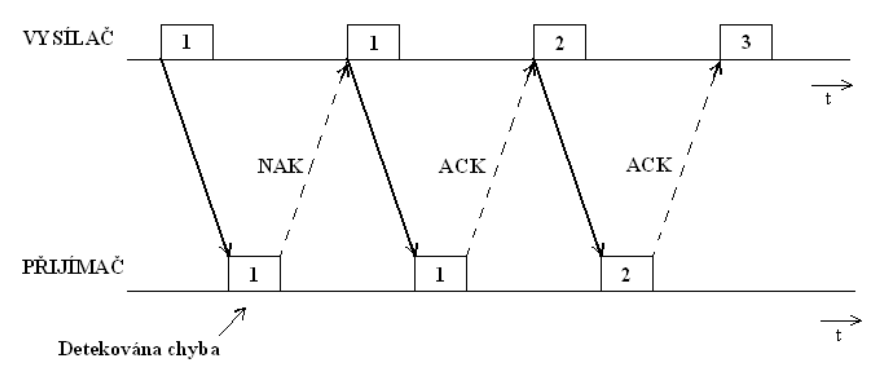
\includegraphics[width=0.9\textwidth]{images/030.png}
\end{figure}

\subsubsection{ARQ Go to n}

ARQ Go to n (návrat k bloku n) zařízení vysílá konstantně bloky přijímači.
Tyto bloky odesílá tak dlouho dokud nepřijde zpráva od přijímače, že obdržel chybný blok.
Po příjmu této zprávy se vysílač vrátí o n bloků a začne vysílat znovu.
Vysílač musí mít uložené odeslané bloky.

\begin{figure}[h]
    \centering
    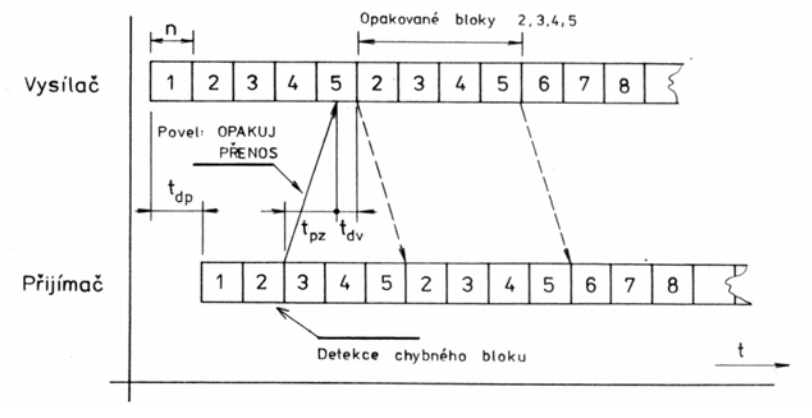
\includegraphics[width=0.9\textwidth]{images/031.png}
\end{figure}

\subsection{ARQ s adresným opakováním}

Tento typ ARQ vychází z ARQ Go to n.
Pokud je nalezene chyba tak se nevrazí o n bloků zpět ale zasílá pouze chybný blok.
Z tohoto je patrné že každý blok musí být označen nějakým identifikátorem (adresa bloku).

\subsubsection{MRQ -- ARQ s pamětí}

Tento princip využívá opakovaného přenosu chybného bloku.
Příjemce chybný blok nezahazuje, jelikož obsahuje některé správné bity.
Příjemce žádá o blok tak dlouho dokud mu nedorazí bezchybný blok nebo dokud si sám blok neumí seskládat z přijatých chybných bloků.
Tento blok je poté kontrolován jako kdyby byl přijat.
Pokud takto sestavený blok je při kontrole vyhodnocen jako správný  nic se neřeší.
Pokud je vyhodnocen jako chybný řeší se to na vyšší systémové úrovni a pravděpodobně bude přenos ukončen kvůli vysoké chybovosti.


\clearpage
\section{Rozdělení protichybových kódů. Schéma realizace procesu kódování blokových kódů a stromových kódů. RM kódy, jejich základní parametry. Obecné blokové schéma kodéru turbokódu, význam jeho částí, dekódování turbokódů. Přehled možností používaných pro zabezpečení proti dlouhým shlukům chyb.}

\subsection{Dělení protichybových kódů}

\begin{figure}[h]
    \centering
    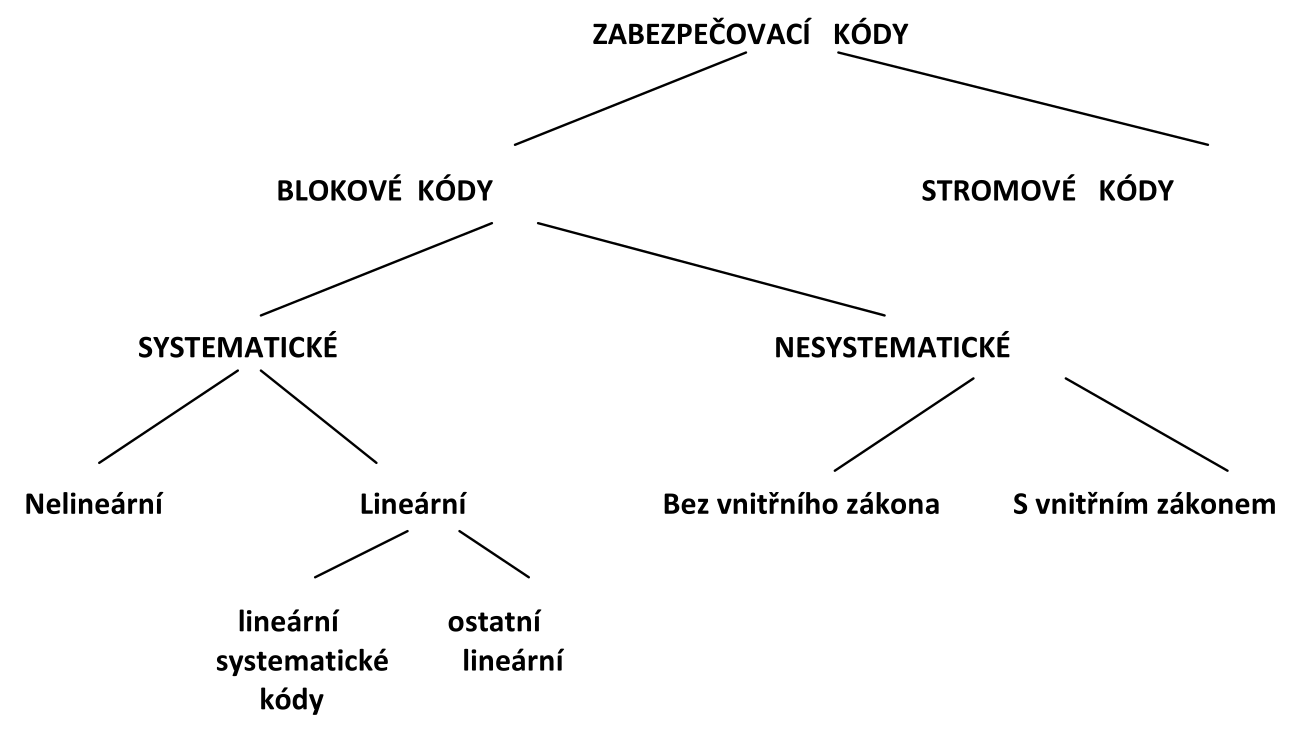
\includegraphics[width=\textwidth]{images/040.png}
\end{figure}

\subsection{Schéma blokových kódů}

\begin{figure}[h]
    \centering
    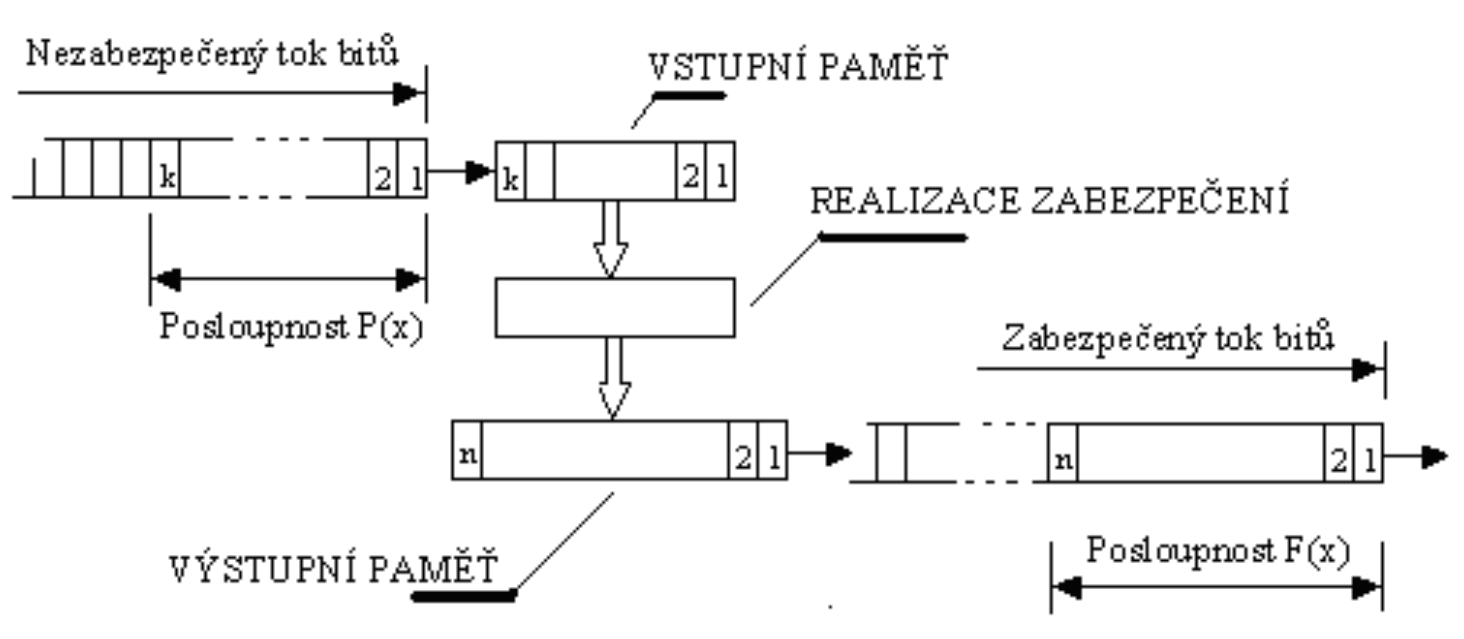
\includegraphics[width=\textwidth]{images/041.png}
\end{figure}

% for subsection to start on new page
\vspace{2cm}

\subsection{Schéma stromových kódů}

\begin{figure}[h]
    \centering
    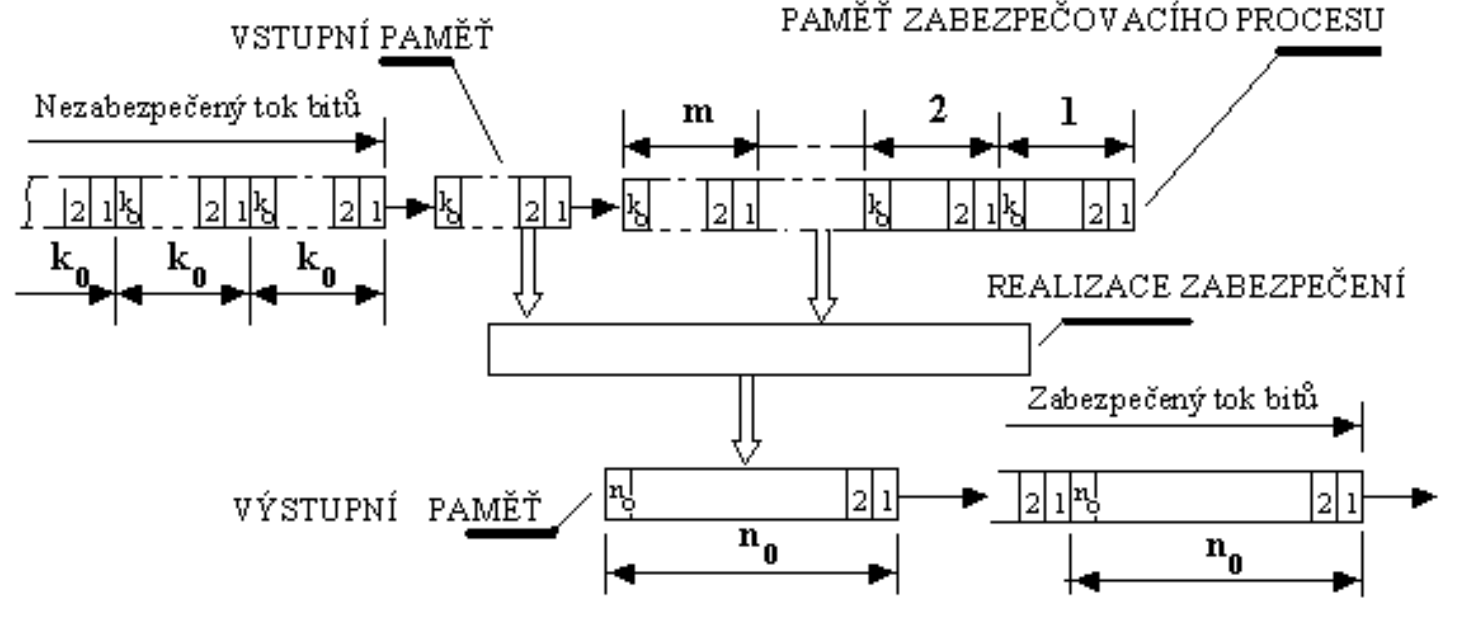
\includegraphics[width=\textwidth]{images/042.png}
\end{figure}

\subsection{Reed Muller kódy (RM kódy)}

RM kódy jsou binární nesystematické kódy, které opravují v kódové kombinaci délky n bitů t nezávislých chyb.
Jejich označení je také R(z;m)

Parametry kódu:

\textbf{Délka kódové kombinace} -- $n = 2^m$\,[bit]

\textbf{Počet nezabezpečených bitů}, které vstupují do zabezpečovacího procesu je určen vztahem 

$k = 1 + k_1 + k_2 + \dots + k_z$ , kde
\[
k=1 +
\begin{pmatrix}
    m \\
    1 \\
\end{pmatrix}
+
\begin{pmatrix}
    m \\
    2 \\
\end{pmatrix}
+
\dots
+
\begin{pmatrix}
    m \\
    z \\
\end{pmatrix}
\]

\textbf{Minimální Hammingova vzdálenost RM kódu} $d_{min} = 2^{m-z}$


\subsection{Turbokódy}

\begin{figure}[h]
    \centering
    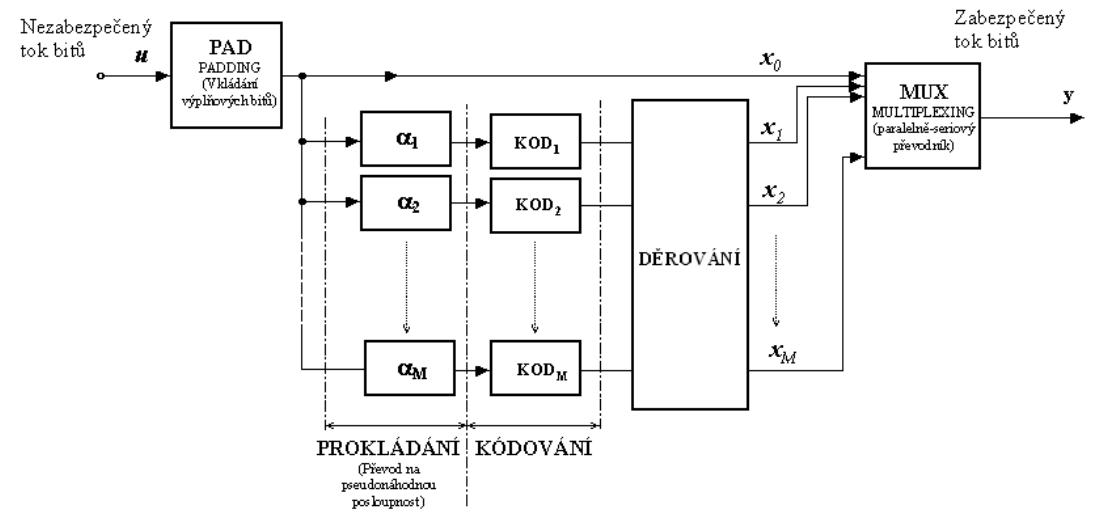
\includegraphics[width=\textwidth]{images/043.png}
\end{figure}

\textbf{Vkládání výplňových bitů (PAD)} -- Za každý datový blok \textit{u} o délce \textit{k} bitů se připojí $(n - k)$ doplňkových bitů.
Toto vytvoří posloupnost $x_0$ bitů.
Posloupnost $x_0$ je převedena na výstup a zároveň paralerně do prokladačů a kodérů.

\textbf{Prokládání} je postup při kterém se původní signálové prvky přeskládají do jiného pořadí.
Každý prokladač převede posloupnost $x_0$ do pseudonáhodného tvaru $\alpha_i$.
Prokladač plní dva úkoly.
Prvním je že vytváří blokový kód (s kodéry) s dlouhou kódovou kombinací.
Druhým úkolem je, že vytváří podmínky pro dekódování.
Změní totiž pořadí bitů pro $KOD_2$ oproti $KOD_1$, $KOD_3$ oproti $KOD_2$, \dots.
Tímto vzniká vysoká pravděpodobnost, že se po opravě některých chyb mohly opravit další některé chyby v dalším dekodéru.

\textbf{Rekurzivní systematické konvoluční kodéry (KOD)} -- Každý kodér poskytuje na svém výstupu zabezpečovací posloupnost $x_i$.
Po určitém počtu kroků je obsah jejich paměťových buněk vymazán.

\textbf{Děrování} se využívá hlavně z důvodu zlepšení informační rychlosti. Děrovaný turbokód pro poměr 1/2 -- první výstupní tok je také první vstupním tokem, ale další výstupní tok je vytvářen multiplexováním výstupů z RSC kodérů.

\subsubsection{Dekódování}

Dekódování je podobné Viterbiho algoritmu.
Na rozdíl od Viterbiho algoritmu, kde je pro výstup pouze možnost 0 nebo 1 pro každý vyhodnocovaný algoritmus, tak turbokody jsou vázány vzájemnou posloupností.
Dekodérů je stejné množství jako kodérů v kódovací části.
Každý dekodér užívá Viterbiho algoritmus s měkkým rozhodováním k vytvoření měkkého rozhodnutí pro každý přijatý bit.

\subsection{Zabezpečení proti shlukům chyb}

\textbf{Možnost změny délky shluku chyb} -- předpokládá se že kód může korigovat i delší shluky chyb $b_{kod}$ než je základní požadavek $b_{min}$.
To představuje rezervu v zabezpečovacích schopnostech kódu. 
Vyjádření rezervy je $\Delta b = b_{kod} - b_{min}$.

\textbf{Možnost změny délky ochranného intervalu} -- Předpokládá se, že kód může mít požadované zabezpečovací schopnosti i při kratším ochranném intervalu, než je požadováno.
Vyjádření změny délky ochranného intervalu $\Delta A = A_{kod} - A_{min}$.


\clearpage
\section{Kryptografické metody zabezpečení datových přenosů, architektura bezpečnosti, služby bezpečnosti, mechanizmy bezpečnosti.}

\subsection{Kryptografické mechanizmy}

\begin{itemize}
    \item Symetrické šifry (blokové, proudové)
    \item Asymetrické (výměna klíče, digitální podpis)
    \item Hašovací funkce
    \item Kryptografické protokoly (SSL, IPsec)
    \item Kvantová a postkvantová kryptografie
    \item Další techniky jako generátor náhodných čísel
\end{itemize}

\subsection{Implementace bezpečnostních funkcí ve vrstvách RM OSI}

Pro implementaci jsou nejvhodnější vrstvy 7. (aplikační protokoly), 4. (transport dat) a 3. (směrovaní).
Bezpečnostní mechanismy jsou zabudovány do aplikačních programů a operačních systémů (7. a 4. vrstva)  a propojovacích zařízení (3. vrstva), ale existují i~způsoby zabezpečení, které využívají další vrstvy.

\subsection{Architektura bezpečnosti v RM OSI}

K zabezpečení se používá doporučení ITU-T X.800, ISO 7498-2 ISO/OSI Security Architecture. Obsahuje mechanismy bezpečnosti (security mechanism), útoky na bezpečnost (security attacks) a službu bezpečnosti (security services), kde jsou definované postupy pro zabezpečení informačních systémů.

\subsection{Služby bezpečnosti}

Služba bezpečnosti je realizovaná protokolem příslušné vrstvy. Existuje 5 kategorií služeb, kterými jsou autentizace (authentication), řízení přístupu (access control), zabezpečení důvěrnosti dat (data confidentiality), zabezpečení integrity dat (data integrity) a ochrana proti odmítnutí původní zprávy (non-repudiation).

\textbf{Autentizace} je proces ověřovaní identity uživatele (entity). Existuje autentizace uživatelů (peer entity authentication), které nezabraňují útoky zopakováním zpráv. Dále existuje autentizace zdroje dat (data origin authentication), která provádí autentizaci všech dat a zabraňuje útokům zopakováním zpráv.

\textbf{Řízení přístupu}: kontrola přístupu (možnost povolit nebo odepřít použití určitého zdroje určitému subjektu, řízení přístupu k materiálním, logickým, nebo digitálním zdrojům; \textbf{neplést si s autorizací}).
Umožňuje přístup  do systému k službám a dalším.
Chrání před neautorizovaným přístupem, kde se nejčastěji nachází v aplikaci nebo OS.

\textbf{Zabezpečení důvěrnosti dat} je ochrana obsahu dat, ochrana toku dat při přenosu proti analýze (zjištění odesílatele, adresáta, \dots). 

\noindent Obsahuje služby pro:
\begin{itemize}[noitemsep]
    \item Důvěrnost přenosu zprávy.
    \item Důvěrnost spojení (ochrana důvěrnosti v rámci navázaného spojení).
    \item Důvěrnost toku dat (chrání informace na zálkadě atributů toku dat).
    \item Selektivní důvěrnosti (ochrana pouze určených částí informace).
\end{itemize}

\textbf{Zabezpečení integrity dat} se zabývá zabezpečením proti neautorizované modifikaci (autorizace je přiřazení oprávnění pro práci v systému, specifikují se činnosti).
Spadají sem služby integrity přenosu zpráv (ochrana integrity všech přenášených zpráv), služba integrity spojení (ochrana přenosů v rámci určitého navázaného spojení) a služby selektivní integrity spojení a selektivní integrity zpráv.
Integritu rozdělujeme na slabou a silnou.

\noindent \textbf{Slabá integrita} slouží pro objevování útoků (modifikace zprávy šumem, náhodná změna pořadí paketů, náhodná duplicita \dots) pomocí aplikací kontrolních součtů, CRC, pořadová čísla paketů atd.

\noindent \textbf{Silná integrita} zabezpečuje proti úmyslným, aktivním útokům (subjektivní útoky) jako jsou podvržení zprávy nebo úmyslné pozměnění zprávy.
Celkově silnou integritu tvoří prostředky slabé integrity a kryptografické prostředky


\textbf{Ochrana proti odmítnutí původu zprávy} zajišťuje důkaz o původnosti dat, prokazuje původ (příjemce, odesílatel) a prokazuje doručení (odesílaní, přijetí).

\vspace{0,5cm}
Celkově by měla být zajištěna autentizace (vím s kým komunikuji) a nepopiratelnost (vím s kým komunikuji a lze to dokázat).

\subsection{Mechanizmy bezpečnosti}

Mechanizmy bezpečnosti jsou šifrování, digitální podpis, řízení přístupu, integrita dat, výměna autentizační informace, padding (výplň), řízení směrovaní a ověření třetím subjektem.


\clearpage
\section{Metalická vedení, náhradní schéma homogenního vedení, primární parametry, sekundární parametry jednotky a vzájemné vztahy. Konstrukce symetrických kabelových vedení používaných v přístupové síti, DM a x čtyřky. Modely elektrických parametrů kabelových vedení určené pro simulaci DSL.}

\subsection{Metalická vedení}

\subsubsection{Základní dělení}

\begin{itemize}
    \item Symetrická vedení -- místní sdělovací kabely, vnitřní rozvody UTP a STP
    \item Nesymetrická vedení -- koaxiální kabely
    \item Silová vedení -- PLC 
\end{itemize}

Nejčastěji tvořeno párem vodičů

\begin{figure}[h]
    \centering
    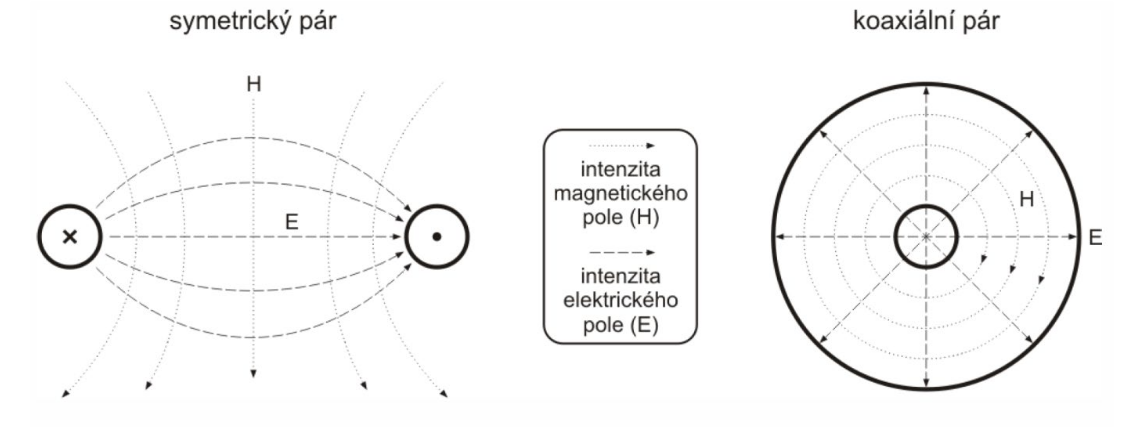
\includegraphics[width=0.6\textwidth]{images/060.png}
\end{figure}

\subsubsection{Schéma homogenního vedení}

\begin{figure}[h]
    \centering
    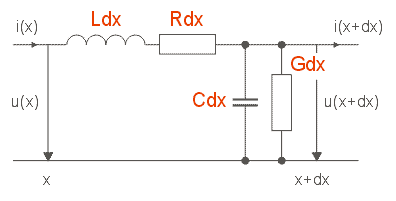
\includegraphics[width=0.5\textwidth]{images/061.png}
\end{figure}

\subsubsection{Primární parametry}
\begin{itemize}
    \item Měrný odpor -- R
    \item Měrná indukčnost -- L
    \item Měrný svod -- G
    \item Měrná kapacita -- C
\end{itemize}

\subsubsection{Sekundární parametry}
\begin{itemize}
    \item Napětí
    \item Proud
    \item Charakteristická impedance
    \item Měrný činitel přenosu
\end{itemize}

\subsection{Mechanická konstrukce kabelů}

Konstrukce kabelů je tvořena kabelovou duší a ochrannými obalu.
Obaly chrání kabelovou duši proti vlivům prostředí a poškození.
Kabel se může skládat s z více vrstev kdy vrstvy jsou oddělené ochranným obalem.

\begin{figure}[h]
    \centering
    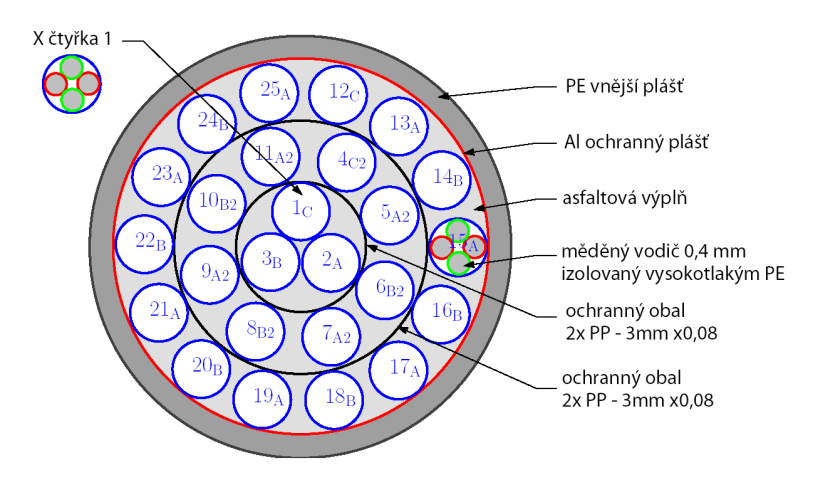
\includegraphics[width=0.5\textwidth]{images/062.png}
\end{figure}

\subsubsection{Čtyřky}
\begin{itemize}
    \item DM čtyřka vzniká stlačením dvou párů s jinou délkou skrutu a oba jsou pak s další délkou skrutu stáčeny dohromady.
    \item Křížová čtyřka je tvořena čtyřmi žílami stočenými se stejnou délkou skrutu.
\end{itemize}

\begin{figure}[h]
    \centering
    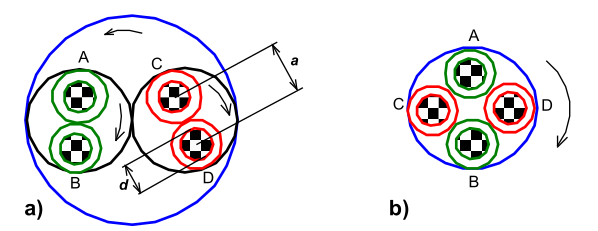
\includegraphics[width=0.5\textwidth]{images/063.png}
\end{figure}

\subsection{Modely kabelových vedení pro simulaci}

\subsection{Modely primárních parametrů}

\begin{itemize}
    \item Analytický tříparametrový model
    \item Numerický devítiparametrový model
    \item Modely British telecom
    \item Modely ITU
    \item Modely Royal PTT Nethrland
\end{itemize}

\subsection{Modely sekundárních parametrů}

\begin{itemize}
    \item Model Deutsche telecom
    \item Model Swisscom
    \item Model Nokia
    \item Modely MAR
\end{itemize}




\clearpage
\section{DSL systémy, vlastnosti, referenční konfigurace, typické uspořádání přípojky, možnosti využití. Základní charakteristiky jednotlivých systémů ADSL, VDSL, vlastnosti, použití.}

\subsection{DSL}

DSL využívá již existujících metalických vedení (telefoní vedení) k přenosu dat.
Nejčastěji je realizován pomocí kroucené dvojlinky.
Existuje několik variant, kterým se souhrnně říká xDSL.
Nejznámějšími zástupci jsou ADSL a VDSL a jejich novější verze (ADSL2, VDSL2) dále to může být SDSL, HDSL nebo SHDSL. 

DSL lze využít například  na připojení k internetu nebo přístup do vzdálené sítě.

\subsubsection{Referenční konfigurace}

NT1 a NT2 jsou síťová zakončení, TA je adaptér pro koncové zařízení.

\begin{figure}[h]
    \centering
    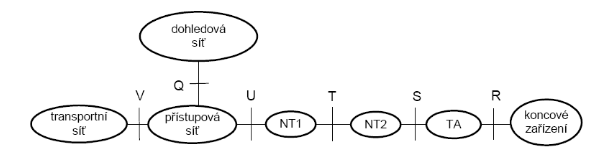
\includegraphics[width=\textwidth]{images/070.png}
\end{figure}

\subsubsection{Uspořádání přípojky}

Nejsem si jistý že je toto, ale je to obecně je to spíše ADSL:

\begin{itemize}
    \item ISP/Poskytovatel
    \item Modem nejčastěji v DSLAM
    \item Splitter
    \item Účastnické vedení
    \item Splitter
    \item Modem
    \item Koncové zařízení uživatele
\end{itemize}

V prezentacích je konfigurace základní přípojky pro ISDN (takže využití IDSL)

\begin{itemize}
    \item zakončení ústředny -- konec zařízení
    \item linkové zakončení -- zabezpečuje přenosové funkce ve veřejné ústředně
    \item opakovač -- je volitelný
    \item síťové zakončení -- zajišťuje fyzické a elektrické podmínky pro připojení koncového zařízení
    \item koncové zařízení
\end{itemize}

\subsection{ADSL}

Používané verze ADSL, ADSL2 a ADSL2+.
Má asymetrické přenosové vlastnosti takže rychlost downstream je vetší jak rychlost upstream.
Rychlosti je možné vidět v tabulce, jsou zde rozšíření všech tří hlavních typů ADSL, které mají trochu vyšší rychlosti rychlosti. ADSL využívá frekvenčního multiplexu (každý kanál má své kmitočtové pásmo) i potlačení ozvěny (echo cancelation -- překrývají se spektra kanálů, možno jenom na nižších frekvencích). Využí se často modulace DMT, kdy každé nosná má šířku 4\,kHz takže vznikne 256 subkanálů.

ADSL využívá frekvenční pásmo 0 až 1,1\,MHz. kdy 0 až 4\,kHz je vyhrazeno pro telefonní přípojku nebo 0 až 80\,kHz pro ISDN přípojku. Zde záleží na využité technice. V případě kombinace s telefonní přípojkou je pro upstream využito pásmo 24 až 138\,kHz a downstream 138 až 1,1\,kHz. V případě ISDN se pásmo jenom posune. 

\begin{table}[ht]
    \centering
    \begin{tabular}{|c|c|c|}
    \hline
        Verze & Downstream\,[Mb/s] & Upstream\,[Mb/s] \\\hline
        ADSL  & 8 & 1 \\\hline
        ADSL2 & 12 & 1 \\\hline
        ADSL2+ & 24 & 1 \\\hline
    \end{tabular}
    \caption{Přehled rychlostí}
\end{table}

ADSL se nejčastěji dá využít pro rychlý přístup do internetu s tím, že je potřeba pouze stahovat.

\subsection{VDSL}

Umožňuje jak symetrické tak asymetrické rychlosti.
Využívá se pro multimediální přístup na internet, distribuci digitálního televizního signálu.
Oproti ADSL má VDSL vyšší přenosové rychlosti.
VDSL využívá 4 pásma v rozsahu 138\,kHz do 12\,MHz.
VDSL2 využívá až 30\,MHz.
Tyto pásma jsou DS1 (směr k účastníkovy), US1 (směrem od účastníka), DS2, UP2.

Maximální dosažené rychlosti pro VDSL jsou 26\,Mb/s v symetrickém režimu a 52/6,4\,Mb/s v asymetrickém.
Na rozdíl od ADSL nevyužívá echo cancelation.
Jelikož je využito vyšší frekvenční pásmo tak rychlost se vzdáleností klesá více než v případě ADSL.


\clearpage
\section{Vliv rušení na provoz xDSL, kategorizace, dosažitelná přenosová rychlost, model přeslechů (NEXT, FEXT), princip výpočtu přeslechů. Spektrální vlastnosti DSL přenosových systémů, správa spektra, cíle, metody.}

\subsection{Vliv rušení}
\begin{description}
    \item[Přeslechy] vznikají při přenosu kabelem, kdy jednotlivé signály xDSL vyzařují energii a ta je pohlcována ostatními páry.
    \item[Provozní šum] je způsoben provozem aktivních a pasivních elektrických prvků. Šum má charakter bílého šumu.
    Není významné.
    \item[Vysokofrekvenční rušení] je způsoben provozem rozhlasových a dalších rádiových systémů.
    Není významné.
    \item [Implusní rušení] je způsobeno různými zdroji produkující krátké elektrické přechodné jevy. Například domácí spotřebiče. 
\end{description}

\subsection{Dosažitelná přenosová rychlost}

Dosažitelná přenosová rychlost vychází ze Shannonova teorému, kdy se přenosová kapacita spočítá jako
\[C = \sum_{i=1}^{N}\frac{B}{N}\log_2(1 + SNR_i(f)),\]
kde B je celková šířka pásma, N je počet subkanálů a SNR je odstup signálu od šumu v i-tém subkanálu.

\subsection{Modely přeslechů}

NEXT je přeslech na blízkém konci a je dominantní v systémech pracující v základním pásmu.
FEXT je přeslech na vzdáleném konci a je dominantní v systémech s kmitočtově odděleným spěrem přenosu (ADSL, VDSL).

\begin{figure}[h]
    \centering
    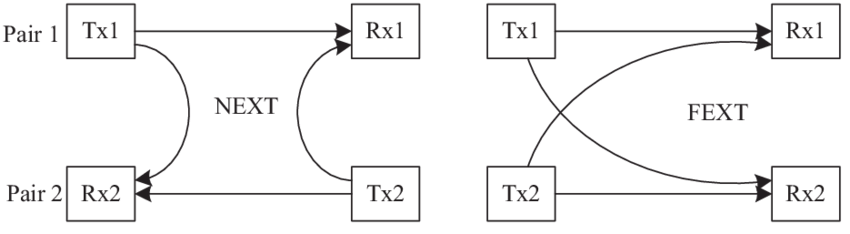
\includegraphics[width=0.6\textwidth]{images/080.png}
\end{figure}

\subsubsection{Výpočet NEXT}

\[|H_{NEXT}(f)| = K_{NEXT} * (\frac{N}{49})^{0,6} * f^{\frac{3}{2}},\]
kde $K_{NEXT} = 8,818 * 10^{-14}$, N je počet zdrojů rušení a $f$ je kmitočet v Hz. 

\subsubsection{Výpočet FEXT}

\[|H_{FEXT}(f)| = K_{FEXT} * (\frac{N}{49})^{0,6} * f^2 * l * |H_{channel}(f, l)|,\]
kde $K_{FEXT} = 8 * 10^{-20}$, N je počet rušících systémů, $f$ je kmitočet v Hz, $|H_{channel}(f, l)|$ je přenosová funkce vedení a $l$ je délka vedení v km.

\subsection{Správa spektra}

Cílem správy spektra je maximální využití kabelové sítě.
Využít spektrum pro maximální počet účastníků a maximální rychlost.

Správa spektra lze dělit na:

\begin{itemize}
    \item Statická -- pevné nastavení parametrů systému při instalaci
    \item Dynamická -- mění se přenosové parametry při provozu
\end{itemize}

Tyto správy lze lze dělit poté do úrovně 0 až 3, kdy úroveň 0 je statická a zbylé 3 úrovně jsou dynamické a sledují různé parametry.

Realizaci správy spektra lze rozdělit dle implementace

\begin{itemize}
    \item autonomní správa
    \item koordinovaná správa -- nejefektivnější
    \item kombinovaná správa
\end{itemize}

Autonomní správa spektra má tři režimy RA (maximální přenosová rychlost), MA (pevná rychlost, maximální výkon) a FM (dosažení garantované rychlosti, využije nezbytný výkon)

Koordinovaná správa spektra potlačuje přeslechy, využívá vectored modulation (VDMT) a vyrovnávání spekter


\clearpage
\section{PLC systémy - praktické využití v energetice - limity technologie, datové objemy, rušení a opakovače. Chytré elektroměry - DLMS protokol a OBIS objekty.}

\subsection{PLC}
\subsubsection{Dělení}

\begin{itemize}
    \item PLC pro velmi vysoká napětí je nejvhodnějším mediem ale není standardizováno
    \item PLC pro vysoká napětí -- používá se pro monitoring a meření
    \item PLC pro nízká napětí je nejpoužívanější, například regulace spotřeby energie, energetické systémy
\end{itemize}

Dále dělíme na:
\begin{itemize}
    \item úzkopásmová PLC -- mají vlastnosti:
    \begin{itemize}
        \item frekvence 3 - 148,5kHz
        \item přenosová rychlost kbit/s
        \item vzdálenost 1-2km
    \end{itemize}
    \item širokopásmové -- mají vlastnosti:
    \begin{itemize}
        \item frekvence 1,6 - 30 MHz
        \item přenosová rychlost Mbit/s
        \item vzdálenost několik stovek metrů
    \end{itemize}
\end{itemize}

\subsubsection{Praktické využití}

Hlavní myšlenkou je že zařízení které nějak komunikuje je většinou připojeno k elektrické síti, takže by bylo vhodné tuto síť využít i pro přenos.

Úzkopásmové PLC systémy lze využít na:
\begin{itemize}
    \item Odečet stavu elektroměrů, plynoměrů, vodoměrů
    \item Centrální sběr dat ze vzdálených snímačů
    \item Alarm, přenos dat a zpětné řízení bezpečnostních kamer
\end{itemize}

\subsubsection{Rušení}

Hlavní zdrojem rušení jsou domácí spotřebiče a další elektrická zařízení.
Rušení může být krátkodobé (zapnutí/vypnutí) nebo trvalé (toto by nemělo nastat).
Další zdroj rušení můžou způsobit jističe, přepěťové ochrany a proudové chrániče. 

\subsubsection{Opakovače}

Opakovače slouží k překlenutí neprůchozí části rozvodné sítě nebo k prodloužení vzdálenosti mezi dvěma PLC modemy.
Opakovač příjme signál ze sítě, zesílí ho a odešle zesílený signál zpátky do sítě.

\subsection{Chytré elektroměry}

Využití chytrých elektroměrů přináší možnost odečtu na dálku.
Hlavní nevýhodou je výrobní/pořizovací cena oproti obyčejným elektroměrům.
Hlavními výhodami jsou:

\begin{itemize}
    \item Dálkový odečet
    \item Monitoring sítě
    \item Dají se snadněji přepínat tarify
\end{itemize}


\subsubsection{DLMS protokol}

DLMS protokol je standardizovaný protokol navržený pro chytré elektroměry.
Umožňuje převádět data z elektroměrů na zprávy.
Je to protokol aplikační vrstvy.

S protokolem DLMS se pojí COSEM standard, který slouží k obecnému popisu modelu objektu.

Spojením DLSM a COSEM vznikne specifikace DLSM/COSEM, který je založen na ISO/OSI.
Tato specifikace popisuje datový model, komunikační protokoly pro výměnu zpráv s měřícím zařízením.
V rámci ISO/OSI DLMS protokol využívá síťovou, transportní a relační vrstvu.
COSEM využívá prezentační vrstvu.
Spojová vrstva má definován protokol HDLC nebo IEC 62056-47.

Skládá se ze tří částí:
\begin{itemize}
    \item Modelování
    \item Zasílání zpráv
    \item Přenos
\end{itemize}

\textbf{Modelování} zahrnuje datový model měřícího zařízení a pravidla pro identifikaci.
Specifikuje vnitřní třídy (IC) COSEM, systém identifikace objektů (OBIS) a použití objektů pro modelování různých funkcí měřičů.

\textbf{Zasílání zpráv} definuje komunikační služby a protokoly pro mapování dat na PDU.

\textbf{Přenos} definuje služby a protokoly pro přenos zpráv.

V DLMS/COSEM klient vždy využívá pro komunikaci logické reference na jméno.
Server je nemusí využívat.
Jsou dva typy referencí -- dlouhé jméno a krátké jméno.

Dlouhé jméno (LN) definuje pro komunikaci klient/server tyto služby:
\begin{itemize}
    \item GET -- získání atributu COSEM třídy objektu
    \item SET -- úprava atributu COSEM třídy objektu
    \item ACTION -- vyvolání metody z COSEM třídy objektu
\end{itemize}

Krátké jméno (SN) definuje tyto služby:
\begin{itemize}
    \item Read -- čtení atributu COSEM třídy objektu
    \item Write -- zápis atributu COSEM třídy objektu (nepředpokládá návratový parameter)
    \item Unconfirmed Write -- zápis atributu COSEM třídy objektu
\end{itemize}

\subsubsection{OBIS Object Identification System}

OBIS poskytuje unikátní identifikátor pro všechny data v měřících zařízeních.
Lze ho použít k identifikaci měřených hodnot, nastavení a získání informací o chování zařízení.
V rámci DLMS/COSEM je OBIS používán dlouhé jméno (LN) pro získání instance objektu COSEM třídy objektu.
OBIS je šestice čísel A až F, kdy každé má svůj význam.

\begin{itemize}
    \item Skupina A -- typ měřené energie nebo média
    \item Skupina B -- udává kanál z ktreého pochází data měření
    \item Skupina C -- Přesná specifikace co se měří
    \item Skupina D -- typ nebo výsledek zpracování fyzikálních veličin ze skupin A-C (min, max, průměr)
    \item Skupina E -- bližší hodnoty měření z A-D
    \item Skupina F -- identifikace historických dat
\end{itemize}

\clearpage
\section{IoT technologie - LoRa, SigFox, NB-IoT.}

LP WAN je reakce na~narůstající počet IoT technologií.
Jsou vhodné pro~omezené uzly (nízká spotřeba, malá cena, dlouhý dosah).
Jejich hlavní nevýhodou je nízká úroveň zabezpečení a nízká datová propustnost.
Jejich použití je vhodné zejména pro~smart metering, pet/property tracking, bezpečnost, smart cities, \dots

Kryptograficky nejsou přenosy chráněny buď vůbec, nebo používají symetrické klíče; asymetrické algoritmy bývají pro~jejich hardware moc náročné.
Některé sítě nabízí i~rotaci klíčů a~E2EE.

\subsection{SigFox, LoRa a NB-IoT -- Společné vlastnosti}

Dobré:
\begin{itemize}[noitemsep]
    \item Nízká energetická spotřeba
    \item Nízká cena
    \item Využití nelicenční sítě
\end{itemize}

Špatné:
\begin{itemize}[noitemsep]
    \item Malá propustnost
    \item Velká hustota připojení na jeden bod
    \item Nelicenční pásmo možné rušení
\end{itemize}

Kriticky špatné:
\begin{itemize}[noitemsep]
    \item Omezený počet společností, nedostatek koncových zařízení
    \item Nepodporuje IP protokol (výjimka NB-IoT)
    \item Bezpečnost sítě
\end{itemize}

\subsubsection{LoRa}

LoRa využívá rádiové technologie, takže výsledné komunikační parametry jsou ovlivněny samostatným přenosem signálu.
Využívá rozprostřeného spektra, takže může komunikovat pod úrovní šumu.
Umožňuje komunikaci na dlouhou vzdálenost pro pásma od 137\,MHz do 1020\,MHz.
Propustnost je v řádech kbit/s.

LoRa k zvýšení odolnosti vůčí rušení a opravě chyb využívá FEC (samoopravný kód, přidávání bitů ke každému datovému bitu)


\subsubsection{SigFox}

Je vhodná pro~sběr dat a senzoriku.
Technologie je navržena tak aby šla vždy přes servery firmy (Francie).
Denní limit 140 zpráv o~velikosti 12~B a čtyři potvrzovací zprávy o~velikosti 8~B.
Využívá DPSK modulace a jedná se o úzkopásmovou technologii s šířkou pásma 200\,Hz.

Pro~zabezpečení používá symetrickou kryptografii; autentizace (Device ID, MAC), integrita (MAC, sekvenční číslo), zabezpečení (není, případně AES-128-CTR).


SigFox komunikace (uplink)

\begin{figure}[h]
    \centering
    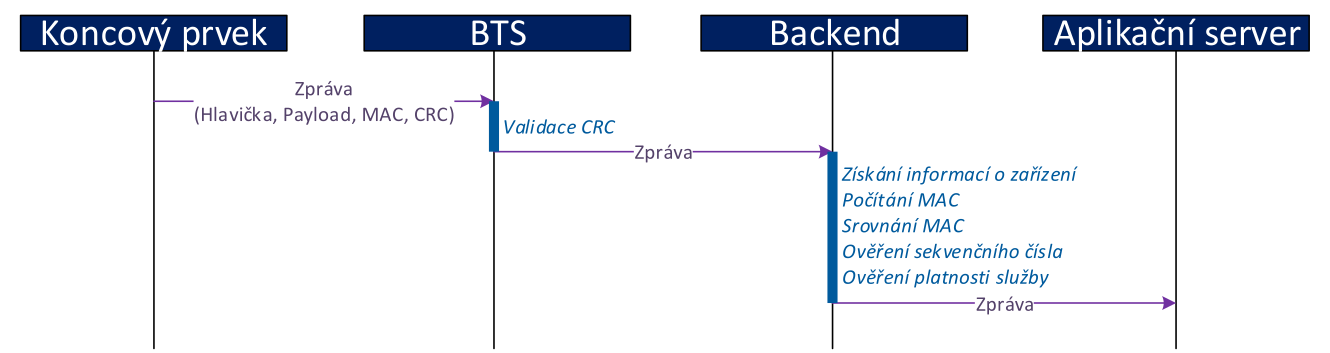
\includegraphics[width=\textwidth]{images/100.png}
\end{figure}


\subsubsection{NB-IoT}

Úzkopásmová LTE komunikace.
50 kbps až 250 kbps s~nízkou latencí.
Náročnější než výše zmíněné (autentizace SIM kartou, vyšší přenosové rychlosti), vyšší cena.
Využívané pásmo má velikost 180\,kHz

Bezpečnost je založena na~3GPP a LTE protokolech uvnitř SIM.
